\section{Finite volume method for Shallow Water Equations}
In this section we will describe the Finite Volume Method (FVM) for solving the shallow water equations (SWE) and the numerical implementation of the method in Python.
In the FVM, we discretize the domain into cells or control volumes.
Then we solve the local Riemann problem at the cell interface to obtain the fluxes.
Using the computed fluxes, we update the solution in each cell.
This way, the FVM allows for discountinuous solutions, as we solve the Riemann problem at the cell interfaces.
Therefore it is well suited for hyperbolic conservation laws, such as the shallow water equations.


\subsection{Finite Volume Methods for the 1D SWE}
We begin by considering finite volume methods for the SWE in one space dimension.
Recall that the homogeneous 1D SWE are given by
\begin{align*}
    h_t + {(hu)}_x &= 0, \\
    {(hu)}_t + {\left(hu^2 + \frac{1}{2}gh^2\right)}_x &= 0.
\end{align*}

A finite volume method for the 1D SWW is based on dividing the spatial domain into a set of intervals, also called grid cells.
The grid is illustrated in Figure~\ref{fig:FVM_1D_grid}.
\begin{figure}[H]
    \centering
    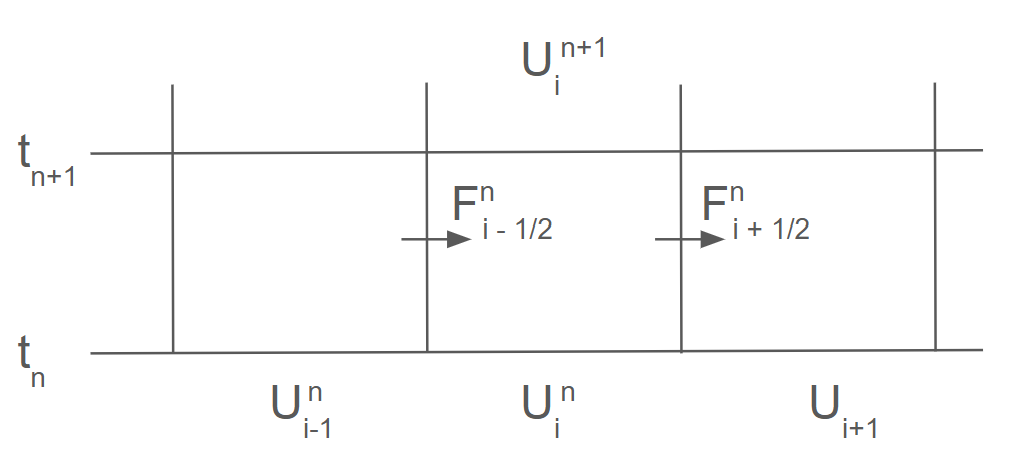
\includegraphics[width=0.5\textwidth]{C:/Users/Matteo/Shallow-Water-Equations/figs/FVM_1D_grid.png}
    \caption{Illustration of the grid for the 1D SWE.}\label{fig:FVM_1D_grid}
\end{figure}

The value $\mathbf{U}_i^n$ approximates the cell average over the $i$-th cell at time $t_n$:
\begin{align}
    \mathbf{U}_i^n \approx \frac{1}{\Delta x} \int_{x_{i-1/2}}^{x_{i+1/2}} \mathbf{U}(x,t_n) dx,
\end{align}
where $\Delta x = x_{i+1/2} - x_{i-1/2}$ is the length of the cell.



Explicit conservative formula 1D SWE
\begin{align}\label{eq:explicit_conservative_1D_SWE}
    \mathbf{U}_i^{n+1} = \mathbf{U}_i^n - \frac{\Delta t}{\Delta x} \left( \mathbf{F}_{i+1/2}^n - \mathbf{F}_{i-1/2}^n \right) + \Delta t \mathbf{S}_i.
\end{align}

This approach~\eqref{eq:explicit_conservative_1D_SWE} is called a finite volume scheme, since it is based on the integral conservation over finite volumes.
Note that the main difference between the FVM and the FDM is that the FVM is based on the integral conservation over finite volumes, whereas the FDM is based on the differential conservation over finite differences.
The main idea in the FVM is to define the numerical flux $\mathbf{F}_{i+1/2}^n$ at the cell inerface as a function of the cell averages $\mathbf{U}_i^n$ and $\mathbf{U}_{i+1}^n$.
Since only the cell-averages solution is known.
This also means that the FVM does not provide pointwise values of the solution, i.e., $\mathbf{U}(x,t)$, but only the cell-averages $\mathbf{U}_i^n$ over the control volume.

\subsection{Finite Volume Method for the 1D SWE with source term}
Consider the inhomoegeneous non-linear system
\begin{align*}
    \mathbf{U}_t + \mathbf{F(U)}_x = \mathbf{S(U)},
\end{align*} 
where $\mathbf{S(U)}$ is a vector of sources. 



\subsection{Finite Volume Method for the 2D SWE}
Follows the methods outlined in~\cite{Toro2009-Riemann}.
Consider a time-dependent two dimensional system of conservation laws
\begin{align}\label{eq:2D_SWE}
    \mathbf{U}_t + \mathbf{F(U)}_x + \mathbf{G(U)}_y = 0.
\end{align}
A numerical explicit finite volume scheme to solve~\eqref{eq:2D_SWE} is given by
\begin{align}
    \mathbf{U}_{i,j}^{n+1} = \mathbf{U}_{i,j}^n + \frac{\Delta t}{\Delta x}(\mathbf{F}_{i-1/2,j} - \mathbf{F}_{i+1/2,j}) + \frac{\Delta t}{\Delta y}(\mathbf{G}_{i,j-1/2} - \mathbf{G}_{i,j+1/2}).
\end{align}
This is the unsplit finite volume method, meaning that, in a single step, the cell average $\mathbf{U}_{i,j}^n+$ is updated using the fluxes from all intercell boundaries.


\subsection{Implementation of the FVM in 1D}
The code to solve the SWE in 1D using FVM is based on the Godunov scheme with the exact Riemann solver.
The exact solution of the Riemann problem is found by using the Riemann invariants and the Rankine-Hugoniot conditions~\cite{trento_course}.

\subsection{Godunov's Method}
We consider the Godunov Upwind method, which is a first-order accurate metod to solve non-linear systems of hyperbolic conservation laws~\cite{Toro2024}.

Consider the initial-boundary value problem (IBVP) for a system of $N$ nonlinear hyperbolic conservation (balance?) laws     
\begin{equation}\label{eq:IBVP_system}
    \begin{cases}
    \text{PDEs: }    &\mathbf{U}_t + \mathbf{F(U)}_x = \mathbf{S(U)}, \quad x \in [a, b], \quad t > 0, \\
    \text{ICs: }    &\mathbf{U}(x,0) = \mathbf{U}^{(0)}(x), \quad x \in [a,b], \\
    \text{BCs: }    &\mathbf{U}(a,t) = \mathbf{B}_{L}(t), \quad \mathbf{U}(b,t) = \mathbf{B}_{R}(t), \quad t \geq 0.
    \end{cases}
\end{equation}
The vectors $\mathbf{B}_L (t)$ and $\mathbf{B}_R (t)$ denote the boundary conditions at the left and right boundaries, respectively.
The Godunov Upwind method in conservative form~\eqref{eq:explicit_conservative_1D_SWE} solves the IBVP~\eqref{eq:IBVP_system}.


\subsection{Implementation of the FVM in 2D}






